\documentclass{standalone}
\usepackage{tikz}

\usetikzlibrary{matrix,positioning,shapes.arrows,fit}

\tikzset{ 
table/.style={
  matrix of nodes,
  row sep=-\pgflinewidth,
  column sep=-\pgflinewidth,
  nodes={
    rectangle,draw,
    text width=0.5cm,
    %minimum width=0.75cm,
    %minimum height=0.75cm,
    align=center},
  text depth=0.125cm,
  text height=0.25cm,
  nodes in empty cells,
  outer sep=0cm,
  },
%texto/.style={font=\footnotesize\sffamily},
%title/.style={font=\small\sffamily}
}

\begin{document}
    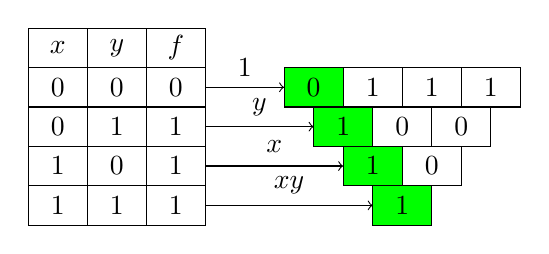
\begin{tikzpicture}[
        every node/.style = {
            draw, rectangle, 
            minimum width=0.75cm,
            minimum height=0.5cm,
            outer sep=0cm, inner sep=0cm,
            node distance=0cm
        }
    ]
    \node (x) {$x$};
    \node [right=of x.east] (y) {$y$};
    \node [right=of y.east] (f) {$f$};

    \node [below=of x.south] (x0) {$0$};
    \node [below=of x0.south] (x1) {$0$};
    \node [below=of x1.south] (x2) {$1$};
    \node [below=of x2.south] (x3) {$1$};

    \node [below=of y.south] (y0) {$0$};
    \node [below=of y0.south] (y1) {$1$};
    \node [below=of y1.south] (y2) {$0$};
    \node [below=of y2.south] (y3) {$1$};
    
    \node [below=of f.south] (f0) {$0$};
    \node [below=of f0.south] (f1) {$1$};
    \node [below=of f1.south] (f2) {$1$};
    \node [below=of f2.south] (f3) {$1$};

    \node [right=1cm of f0.east, fill=green] (r00) {0};
    \node [right=of r00.east] (r01) {1};
    \node [right=of r01.east] (r02) {1};
    \node [right=of r02.east] (r03) {1};

    \node [below=of r00.south east, fill=green] (r10) {1};
    \node [right=of r10.east] (r11) {0};
    \node [right=of r11.east] (r12) {0};

    \node [below=of r10.south east, fill=green] (r20) {1};
    \node [right=of r20.east] (r21) {0};

    \node [below=of r20.south east, fill=green] (r30) {1};

    \draw [->] (f0.east) -- node[draw=none, above] {1} (r00.west);
    \draw [->] (f1.east) -- node[draw=none, above] {$y$} (r10.west);
    \draw [->] (f2.east) -- node[draw=none, above] {$x$} (r20.west);
    \draw [->] (f3.east) -- node[draw=none, above] {$xy$} (r30.west);
    \end{tikzpicture}
\end{document}